\section{Why AES works? -- The mathematical foundations}
\label{sec:why}
\label{sec:math}

Figure \ref{fig:aes-round-function} shows the graph of a single AES round. 
The 16-byte input $A_0, \dots, A_{15}$ is fed byte-wise into the S-Box in the Byte Substitution Layer (Section \ref{sec:byte-substitution}).
The 16-byte output $B_0, \dots, B_{15}$ is permutated twice in the \textsc{ShiftRows} layer and mixed by the \textsc{MixColumn} transformation, both in the Diffusion layer (Section \ref{sec:diffusion})
Finally, the 128-bit subkey $k_i$ is XORed with the immediate result in the Key Addition layer (Section \ref{sec:key-addition}).

The mathematical foundations discussed in subsequent subsections are based on the \gls{AES} specification published by \gls{NIST} \cite{NIST_AES} and the textbook by Paar and Pelzl \cite{Paar2024}.

\begin{figure}[!ht]
    \centering
    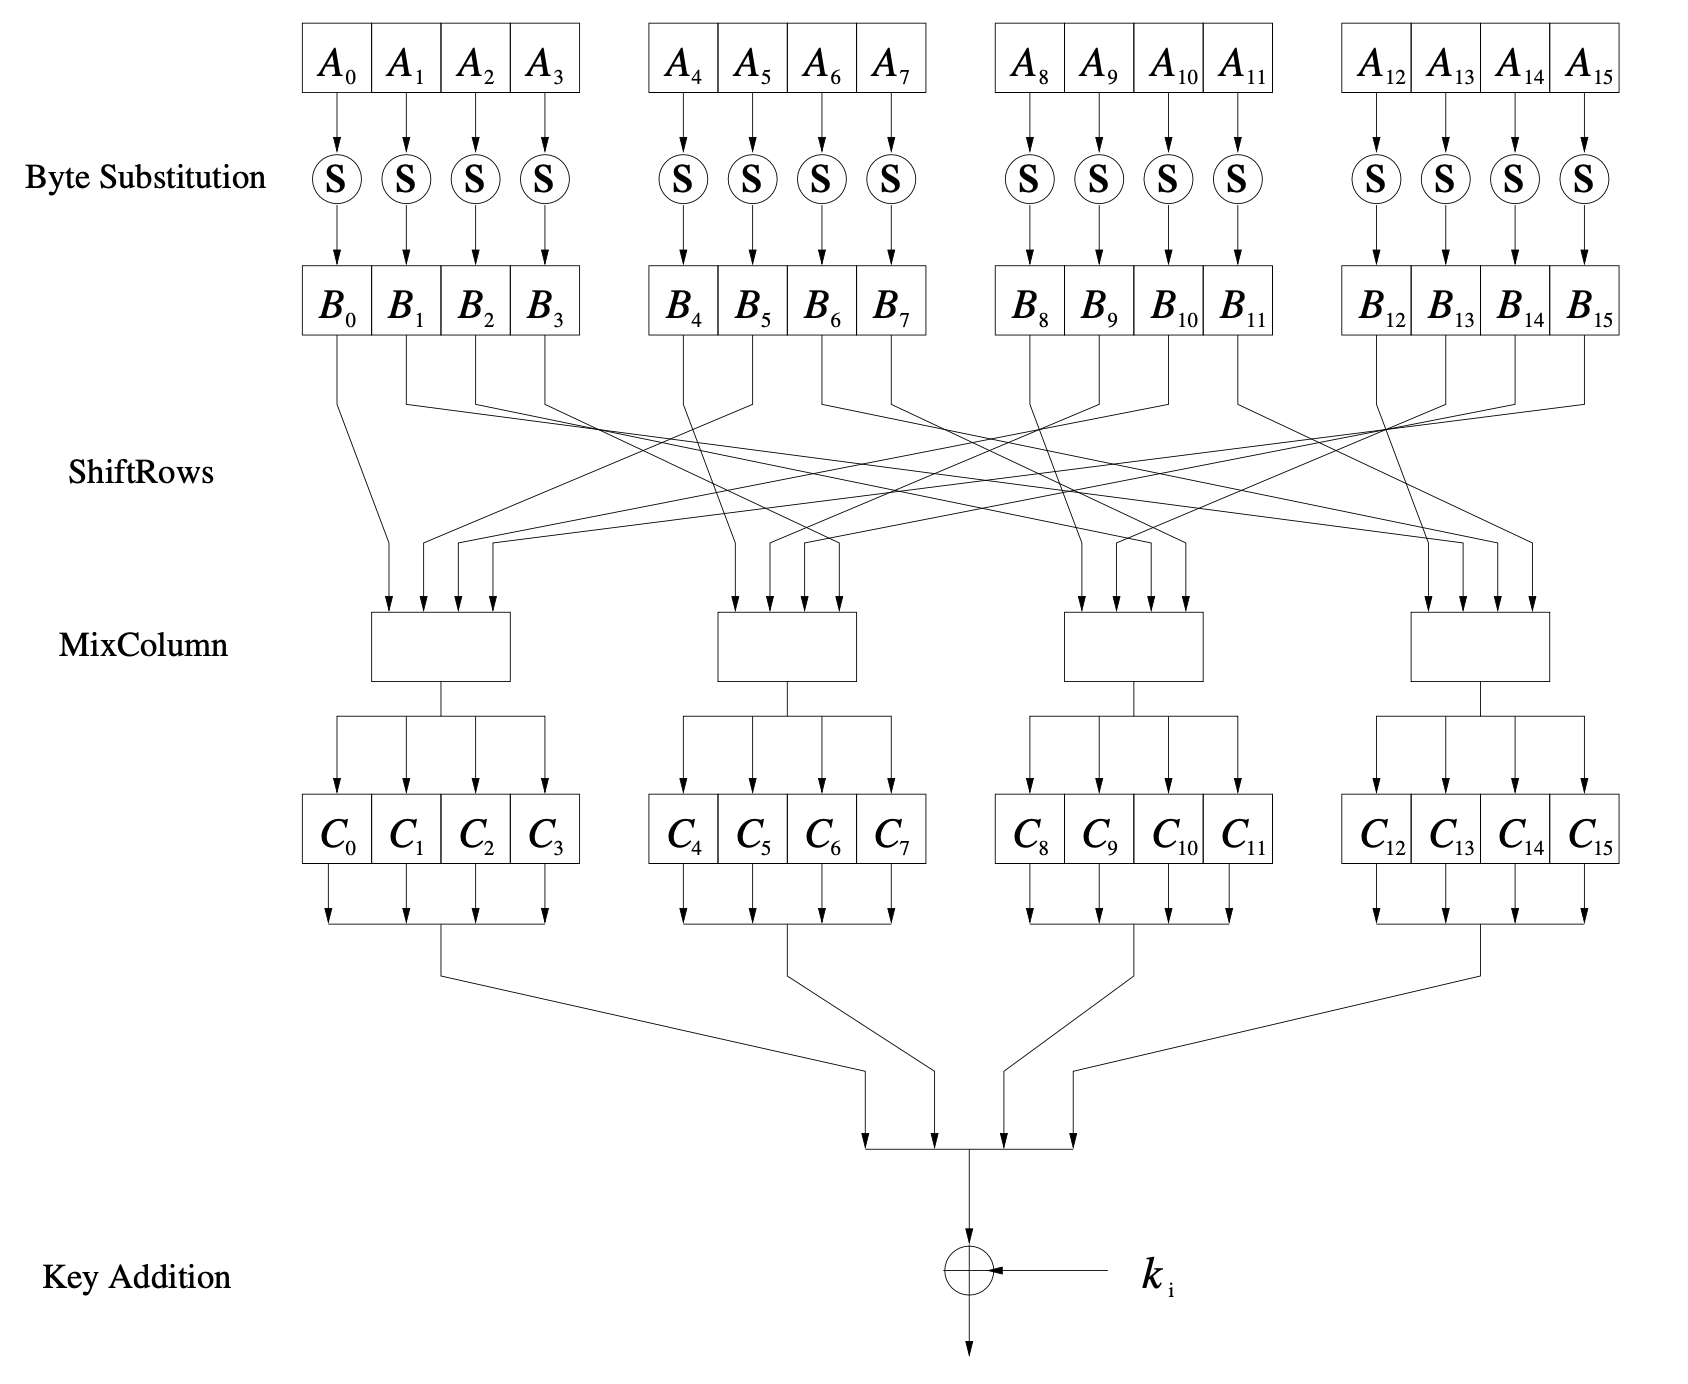
\includegraphics[width=.9\textwidth]{aes-round-function.png}
    \caption{
        AES round function for rounds $1, 2, \dots, n_r-1$ \cite{Paar2024}.
    }
    \label{fig:aes-round-function}
\end{figure}


\subsection{Mathematical Preliminaries}



\subsubsection{Addition}
\label{sec:addition}



\subsubsection{Multiplication}
\label{sec:multiplication}

\subsection{\textsc{SubBytes} transformation}
\label{sec:SubBytes}

The Byte Substitution layer can be viewed as a row of 16 parallel S-Boxes, each with 8 input and output bits (see Figure \ref{fig:aes-round-function}). 
Each state byte $A_i$ is replaced, i.e. substituted, by another byte $B_i$.

\begin{figure}[!ht] 
    \centering
    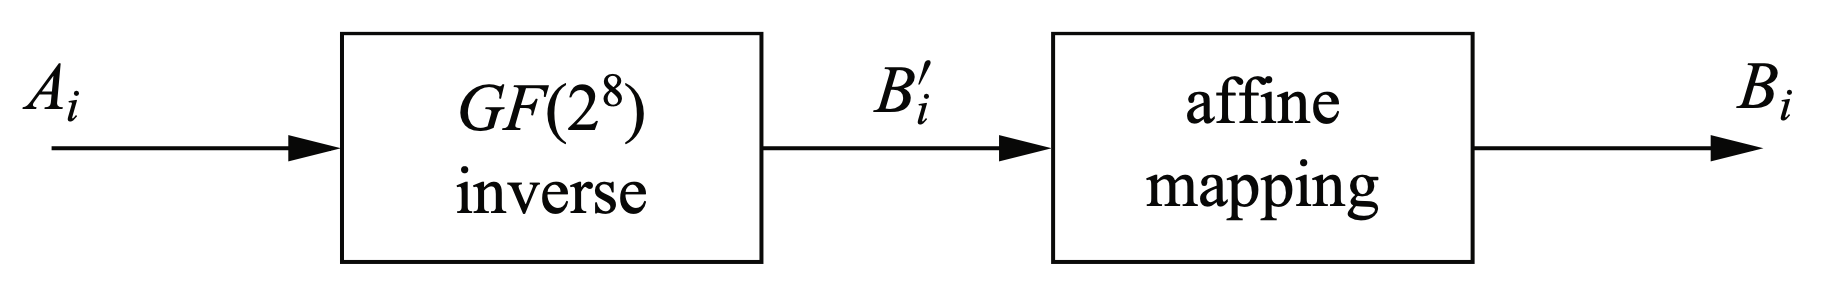
\includegraphics[width=.6\textwidth]{byte-substitution.png} 
    \caption{
        The two operations within the AES S-Box which computes the function $B_i = S(A_i)$ \cite{Paar2024}.
    }
    \label{fig:byte-substitution} 
\end{figure}

The \textsc{SubBytes} transformation is a non-linear byte substitution that operates independently on each byte of the state byte.
The S-Box is constructed by composing of two transformation:
\begin{enumerate}
    \item \textbf{Galois Field Inversion}: 
    Take the multiplicative inverse in the finite field $GF(2^8)$ and solve for ${B'}_i$ (Equation \ref{eq:gfi}), described in Section \ref{sec:multiplication}. 
    The element $\{00\}$ is mapped to itself.
    
    \begin{align}
        A_i \cdot {B'}_i &= 1 \mod P(x)
        \label{eq:gfi}
    \end{align}

    \item \textbf{Affine Mapping}:
    
    The following affine transformation (over $GF(2)$) is applied:
    \begin{align}
        b_i = {b'}_i \oplus {b'}_{(i+4 \mod 8)} \oplus {b'}_{(i+5 \mod 8)} \oplus {b'}_{(i+6 \mod 8)} \oplus {b'}_{(i+7 \mod 8)} \oplus c_i
    \end{align}
    for $0 \leq i \leq 8$, where $b_i$ is the $i$-th bit of the byte and $c_i$ is the $i$-th bit of a byte $c$ that is to be transformed.

    % Apply the following transformation with
    % each byte ${B'}_i$ is multiplied by a constant bit-matrix, followed by the addition of a constant 8-bit vector:
    % \begin{align}
    %     \begin{pmatrix}
    %         1 & 0 & 0 & 0 & 1 & 1 & 1 & 1\\
    %         1 & 1 & 0 & 0 & 0 & 1 & 1 & 1\\
    %         1 & 1 & 1 & 0 & 0 & 0 & 1 & 1\\
    %         1 & 1 & 1 & 1 & 0 & 0 & 0 & 1\\
    %         1 & 1 & 1 & 1 & 1 & 0 & 0 & 0\\
    %         0 & 1 & 1 & 1 & 1 & 1 & 0 & 0\\
    %         0 & 0 & 1 & 1 & 1 & 1 & 1 & 0\\
    %         0 & 0 & 0 & 1 & 1 & 1 & 1 & 1
    %     \end{pmatrix}
    %     \begin{pmatrix}
    %         {b'}_0\\
    %         {b'}_1\\
    %         {b'}_2\\
    %         {b'}_3\\
    %         {b'}_4\\
    %         {b'}_5\\
    %         {b'}_6\\
    %         {b'}_7
    %     \end{pmatrix}
    %     +
    %     \begin{pmatrix}
    %         1\\
    %         1\\
    %         0\\
    %         0\\
    %         0\\
    %         1\\
    %         1\\
    %         0
    %     \end{pmatrix}
    %     &\equiv
    %     \begin{pmatrix}
    %         b_0\\
    %         b_1\\
    %         b_2\\
    %         b_3\\
    %         b_4\\
    %         b_5\\
    %         b_6\\
    %         b_7
    %     \end{pmatrix}
    % \end{align}
    % where ${B'_i} = \left( {b'}_0, \dots, {b'}_7 \right)$ and $B_i = \left( b_0, \dots, b_7 \right)$
\end{enumerate}

% A lookup table for the \textsc{SubBytes} transformation can be generated by computing the substitution values for all possible two-digit hexadecimal inputs (i.e., 256 values from \texttt{00} to \texttt{FF}).
\textcolor{red}{insert lookup table}
\subsection{\textsc{ShiftRows}}

The \textsc{ShiftRows} transformation cyclincally shifts the second row of the state matrix three bytes to the right, the third row by two bytes to the right, and the forth row by one byte to the right (Eq. \ref{eq:ShiftRows}).
The first row is not changed.

The purpose of this is to increase the diffusion properties of AES.

\begin{equation}
    \begin{array}{c@{\quad \longrightarrow \quad}c}
        \begin{array}{|c|c|c|c|}
        \hline
        B_0 & B_4 & B_8 & B_{12} \\
        \hline
        B_1 & B_5 & B_9 & B_{13} \\
        \hline
        B_2 & B_6 & B_{10} & B_{14} \\
        \hline
        B_3 & B_7 & B_{11} & B_{15} \\
        \hline
        \end{array}
    &
    \begin{array}{|c|c|c|c|}
        \hline
        B_0 & B_4 & B_8 & B_{12} \\
        \hline
        B_5 & B_9 & B_{13} & B_1 \\
        \hline
        B_{10} & B_{14} & B_2 & B_6 \\
        \hline
        B_{15} & B_3 & B_7 & B_{11} \\
        \hline
        \end{array}
    \end{array}
    \label{eq:ShiftRows}
\end{equation}
\subsection{\textsc{MixColumns}}

The \textsc{MixColumn} transformation is a linear transformation which mixes each column of the state matrix. 
\begin{align}
    MixColumn(B) &= C\\
    \begin{pmatrix}
        02 & 03 & 01 & 01\\
        01 & 02 & 03 & 01\\
        01 & 01 & 02 & 03\\
        03 & 01 & 01 & 02
    \end{pmatrix}
    \cdot
    \begin{pmatrix}
        B_{0,c} \\
        B_{1,c} \\
        B_{2,c} \\
        B_{3,c} \\
    \end{pmatrix}
    &=
    \begin{pmatrix}
        C_{0,c} \\
        C_{1,c} \\
        C_{2,c} \\
        C_{3,c} \\
    \end{pmatrix}
\end{align}
for $0 \leq c \leq Nb$.
% with $B$ being the 16-byte input state after \texttt{ShiftRows} operation given in Equation \ref{} and C being the 16-byte output state.
% Each vector column of B is multiplied by a fixed $4 \times 4$ matrix (containing constant entries).

As a result of this multiplication, the four bytes in a column are replaced with the following
\begin{align}
    C_{0,c} & = (\{02\} * B_{0,c}) &&\oplus (\{03\} * B_{1,c}) &&\oplus B_{2,c} &&\oplus B_{3,c}\\
    C_{1,c} & = B_{0,c} &&\oplus (\{02\} * B_{1,c}) &&\oplus (\{03\} * B_{2,c}) &&\oplus B_{3,c}\\
    C_{2,c} & = B_{0,c}  &&\oplus B_{1,c} &&\oplus (\{02\} * B_{2,c}) &&\oplus (\{03\} * B_{3,c})\\
    C_{3,c} & = (\{03\} * B_{0,c}) &&\oplus B_{1,c} &&\oplus B_{2,c} &&\oplus (\{02\} * B_{3,c})
\end{align}

\subsection{\textsc{AddRoundKey} transformation}
\label{sec:AddRoundKey}

The \textsc{AddRoundKey} transformation combines the current state matrix with a round key derived from the key expansion process (Section \ref{sec:key-expansion}). 

This transformation operates by performing a bitwise \texttt{XOR} operation between each byte of the state matrix and the corresponding byte of the round key, represented as:
\begin{equation}
    C_{i,\text{out}} = C_{i,\text{in}} \oplus K_i
\end{equation}
where $ C_{i,\text{in}}$ and $C_{i,\text{out}}$ denote the input and output bytes of the state respectively, and $K_i$ represents the corresponding byte of the round key.

This step introduces key-dependent confusion into the encryption process, ensuring that the state is uniquely modified at each round based on the key material.
\subsection{Key Expansion (Key Schedule)}

\subsubsection*{Importance of Key Expansion in AES} 

The Advanced Encryption Standard (AES) heavily relies on the key expansion (or key schedule), 
a process that derives a series of round keys from the initial cipher key. 
This process ensures that each round uses a different key, 
greatly increasing the cipher's security. The key expansion process slightly differs 
based on the AES version (AES-128, AES-192, or AES-256), mainly in the number of rounds 
and the size of the key.

\subsubsection*{Main Algorithm of Key Expansion}

First, the initial key is loaded into the first $N_k$ words of the key schedule, where $N_k$ depends 
on the key size $K_{len}$ and the number of rounds $N_r$: ($K_{len}$, $N_r$) = (128, 10), (192, 12), and (256, 14) 
for AES-128, AES-192, and AES-256, respectively \cite{Key_Collisions} (shown in Figure~\ref{fig:key_comb}). AES requires $N_r+1$ round keys, each round key is 
128 bits (16 bytes) in size, equivalent to four words $N_b$ from the key schedule. The key schedule in 
response generates a total of $N_b$×($N_r+1$) words\cite{NIST_AES}. \newline

For example, for AES-192, the key schedule generates 52 words in the key expansion, which equals 208 bytes (4 \textit{bytes per word} × 52 \textit{words}).
13 round keys are then extracted from these words - one for each of the 12 rounds plus the initial key addition ($N_r$ + 1 = 13).

\begin{figure}[h] % 'h' means place the figure here if possible
    \centering
    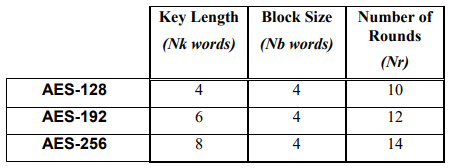
\includegraphics[width=.8\textwidth]{197_key_combinations.png} % Adjust width as needed
    \caption{
        Key-Block-Round Combinations \cite{Standards2001}
    }
    \label{fig:key_comb} % Reference this figure with \ref{fig:sample_image}
\end{figure}

Then, the remaining words are generated iteratively. For words at positions that are a multiple of $N_k$, a 
transformation is applied to the previous word w[i-1] before the \Gls{XOR}. This transformation consists of RotWord 
followed by SubWord, and the result is then XORed with a round constant Rcon[i], where:

\begin{enumerate}
    \item \textbf{RotWord}: A cyclic permutation that shifts the bytes in the 4-byte input word one position to the left. 
    \item \textbf{SubWord}: A substitution operation that applies SubBytes operation to a 4-byte input word. 
    \item \textbf{Round Constant (Rcon)}:  An \Gls{XOR} operation with a round-dependent constant RC, where each Rcon[i]
    has a structure (RC[i], 0x00, 0x00, 0x00) \cite{Standards2001}. 
\end{enumerate}

If the AES version is AES-256 ($N_k$ = 8) and i-4 is a multiple of $N_k$, the SubWord transformation is applied to the 
previous word (shown in Figure), but RotWord and Rcon are skipped. Otherwise, the new word is generated by XORing the previous word 
with the word $N_k$ positions earlier in the key schedule \cite{Standards2001}. 

\begin{figure}[h] % 'h' means place the figure here if possible
    \centering
    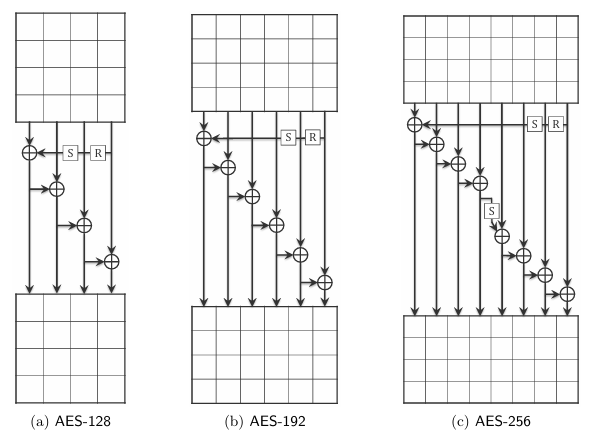
\includegraphics[width=.8\textwidth]{key_schedules.png} % Adjust width as needed
    \caption{
        Key schedules of AES-128, AES-192, and AES-256.The SubWord and
        RotWord functions are denoted by $S$ and $R$, respectively. Note that the round
        constant is not shown. \cite{Key_Collisions}
    }
    \label{fig:key_comb} % Reference this figure with \ref{fig:sample_image}
\end{figure}

\begin{figure}[h]
    \centering
    \includegraphics[width=.8\textwidth]{key_schedule-128.png}
    \caption{Key schedule for AES-128 \cite{Paar2024}.}
    \label{fig:key-schedule-128}
\end{figure}

\subsubsection*{Key Size and Security}

The key size directly impacts the security level of the algorithm, with 
longer keys providing higher security against brute force attacks. AES-128 offers sufficient security 
for most applications, but AES-192 and AES-256 are often preferred for applications requiring 
long-term security or protecting highly sensitive data. The increased number of rounds in AES-256 
further enhances its resistance against advanced cryptanalytic techniques.
\subsection{Security Properties}

Modes of operation define how a block cipher like AES is applied to variable-length data. 
Each mode introduces distinct security implications, 
including confidentiality, error propagation, resistance to structural analysis, 
and resilience against future threats such as quantum computing.

\noindent The security of a mode depends not only on AES itself but also on how the blocks are processed. 
For instance:

\begin{itemize}
    \item \textbf{\Gls{ECB} Mode} encrypts each block independently, leading to pattern leakage. Identical plaintext blocks produce identical ciphertexts, compromising confidentiality, especially in structured data like images.
    
    \item \textbf{\Gls{CBC} Mode} introduces randomisation through an \Gls{IV}, ensuring that identical messages yield different ciphertexts. However, encryption is inherently sequential and more sensitive to bit-flip propagation.
    
    \item \textbf{\Gls{CFB} and \Gls{OFB} Modes} convert the block cipher into a stream cipher. OFB offers better error isolation, while CFB is self-synchronising but more susceptible to feedback-based error propagation.
    
    \item \textbf{\Gls{CTR} Mode} enables full parallelism and random access by encrypting incrementing counters. It avoids feedback loops and supports high-throughput use cases, making it robust in environments requiring speed and scalability.
    
    \item \textbf{\Gls{XTS}-AES} is optimised explicitly for disk encryption. It uses a tweakable block cipher based on sector position to ensure that the same data encrypted at different locations yields different ciphertexts, offering strong structural and positional integrity.
\end{itemize}

With the anticipated rise of quantum computing, 
AES modes must also be evaluated under quantum threat models. 
Grover’s algorithm reduces brute-force complexity from $2^k$ to approximately $2^{k/2}$. \newline

Jang et al.\cite{Jang2025} present refined circuit depth and gate count estimates under realistic quantum constraints. 
Their study indicates the following effective quantum security levels:

\begin{itemize}
    \item AES-128: $2^{156.26}$
    \item AES-192: $2^{221.58}$
    \item AES-256: $2^{286.07}$
\end{itemize} 

These values, derived using optimised Grover-based search circuits, 
are well above the estimated practical capabilities of near-term quantum computers\cite{Jang2025}. \newline

Importantly, parallelisable modes like CTR and XTS are more amenable to low-depth quantum circuit implementations. 
Their compatibility with constraints such as NIST’s \texttt{MAXDEPTH} parameter makes them promising candidates for quantum-resilient applications\cite{Jang2025}.

\begin{table}[h]
\centering
\resizebox{\textwidth}{!}{%
\begin{tabular}{|l|c|c|c|l|}
\hline
\textbf{Mode} & \textbf{Parallel} & \textbf{Error Propagation} & \textbf{Random Access} & \textbf{Best Use Case} \\
\hline
\Gls{ECB} & Yes & None & Yes & Toy cases, testing only \\
\Gls{CBC} & No (Enc) / Yes (Dec) & Yes(next block) & No & File encryption \\
\Gls{CFB} & No & Yes(next block) & No & Streaming data with feedback \\
\Gls{OFB} & Yes & None & No & Resilient byte-wise streaming \\
\Gls{CTR} & Yes & None & Yes & High-throughput systems \\
\Gls{XTS} & Yes & None & Yes & Secure disk encryption \\
\hline
\end{tabular}%
}
\caption{Security characteristics of AES modes of operation.}
\end{table}

